


\section{Two-layer Cuckoo Hash}\label{sec:vot}
In this section, we present a two-layer approach that ensures a maximum of two lookups for \formal{find} and \formal{delete} (Section~\ref{sec:vot:two}). 
Subsequently, in Section~\ref{sec:vot:con}, we give details on optimizing GPUs for paralleling hash table operations such as \formal{find}, \formal{insert}, and \formal{delete}.


%\begin{algorithm}[t]
%	\begin{algorithmic}[1]
%		\State $found \gets \emptyset$
%		\For{$i=0,\ldots,d-1$}
%		\State $loc \gets h^i(k)$
%		\State $found \gets ballot(loc[l].key == k)$
%		\If{$found \neq \emptyset$}
%		\State \Return $loc[l]$
%		\EndIf
%		\EndFor
%		\State \Return false
%	\end{algorithmic}
%	\caption{\textbf{Find}(lane $l$, warp $wid$, key $k$)}\label{algo:find}
%\end{algorithm}

\subsection{The Two-layer Approach}\label{sec:vot:two}
Given the proposed dynamic hash table design, a larger $d$ implies a smaller workload for each resizing operation, as each single table will be smaller with fixed filled factor. In addition to efficient resizing, a higher filled factor can be maintained for a larger $d$ as discussed in Section~\ref{sec:dyn:resize}. Nevertheless, the benefit of employing more tables does not come for free. For each \formal{find} and \formal{delete} operations, one must perform $d$ lookups, which translates to $d$ random accesses to the device memory. 
Random accesses are particularly expensive as GPUs contain limited cache size and simplified control units compared to CPUs.

One possible approach to reduce the number of lookups is to first hash all KV pairs into $d'$ partitions. For each partition, we employ a cuckoo hash with two hash functions. In this manner, one only performs at most two lookups for any \formal{find} and \formal{delete} operations. However, this approach cannot prevent skewness across the $d'$ partitions, especially with frequent delete operations. It is possible that the deleted KVs all fall into one partition $c_i$, which results in low filled factor for the table or tables allocated to $c_i$. Furthermore, when inserting KVs into other partitions, e.g., $c_j \neq c_i$, efficiency could be severely degraded due to the high filled factor of the table or tables allocated to $c_j$. 

Hence, we propose a two-layer approach to resolve the skewness problem.
\revise{
The two-layer approach is inspired by data partitioning techniques~\cite{bender2012don,boncz1999database,zhang2019data,zuo2018write}. 
}
Given $d$ hash tables, we first hash all KV pairs into $\binom{d}{2}$ partitions, 
each of which refers to a unique pair of hash tables. Then each KV pair is hashed and stored in only one of the corresponding pair. This only requires a maximum of two lookups for \formal{find} and \formal{delete}. The advantage of this approach is that each KV pair could appear in any of the $d$ hash tables, which provides opportunities to balance a skewed distribution. The following example illustrates a scenario where skewness is mitigated during the insertion process. 

\begin{example}
A KV pair $(k,v)$ is hashed to the hash table pair $(h_i,h_j)$ for the first layer. We then hash $k$ and try to insert $(k,v)$ into $h_i$ for the second layer. Assuming the corresponding bucket in $h_i$ is full for $(k,v)$, we evict another KV pair $(k',v')$. We then discover that $(k',v')$ is hashed to the pair $(h_i,h_t)$. Henceforth, we insert $(k',v')$ to $h_t$ and the process repeats until no further evictions occur.
\end{example}

The above example shows that the eviction could reinsert a KV pair into any hash table $h_t$. As each filled bucket contains 32 KV pairs (assuming 4 byte keys), one can pick a KV pair for reinsertion into a desired hash table based on the balancing strategy discussed in Theorem~\ref{them:balance}. In addition to the ability to mitigate data skewness, the two-layer cuckoo hash has the same asymptotic insertion performance as a plain cuckoo hash table with two hash functions.  

\begin{theorem}\label{them:complexity}
The two-layer cuckoo hash approach has the same expected, amortized complexity of insertions as a plain cuckoo hash with two hash tables. 
\end{theorem}

\begin{proof}
Assuming $d$ hash tables for the two-layer approach, without loss of generality we set the range for each hash function to be $[0,n)$. Given a KV pair $(k,v)$, we denote hash function $hp$ as the one that hashes $(k,v)$ to a pair of hash tables.
Now, we transform the two-layer approach to the plain cuckoo hash by constructing two new hash functions $H_1(k) = i \cdot n \cdot h_i(k)$ and $H_2(k) = j \cdot n \cdot h_j(k)$ where $hp(k) = (h_i,h_j)$.
The apparent range of $H_1$ and $H_2$ is $[0,nd)$. Thus, we can build a random bipartite graph $G(U,V,E)$, where $U$ represents the buckets for $H_1$, $V$ represents the buckets for $H_2$, and $E$ represents the KV pairs connecting the two buckets from $H_1$ and $H_2$. 
Each KV pair is independently hashed to a random edge $e \in E$ with the same probability, i.e., $1/(n^2d^2)$. Hence, we can follow a similar proof procedure that utilizes random bipartite graph analysis to show the amortized complexity of a cuckoo hash with two tables \cite{kutzelnigg:hal-01184689}, to prove Theorem~\ref{them:complexity}.
\end{proof}



\subsection{Parallel Hash Table Operations}\label{sec:vot:con}
In the reminder of this section, we discuss how to utilize GPUs for the two-layer cuckoo hash. Following existing works \cite{alcantara2009real,zhang2015mega,breslow2016horton}, we assume that the \formal{find}, \formal{insert} and \formal{delete} operations are batched and that each batch contains only one type of operations. 
%A batch with mixed type of operations can also be supported but the semantic is ambiguous. 

\begin{figure}[t]
	\centering
	\hspace{-3em}
	\begin{minipage}{0.5\linewidth}
		\label{fig:atomicCAS}
		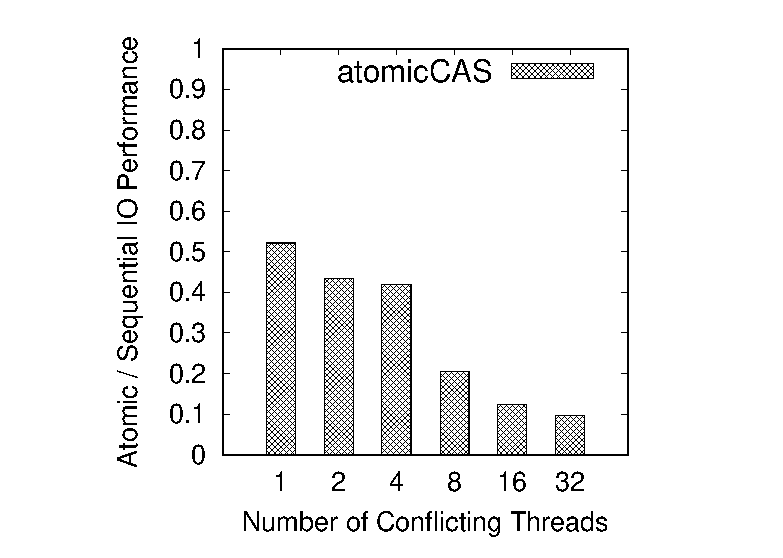
\includegraphics[width=5.3cm]{exp/atomic/atomicCAS.eps}
	\end{minipage}
	\hspace{-1em}
	\begin{minipage}{0.5\linewidth}
		\label{fig:atomicExch}
		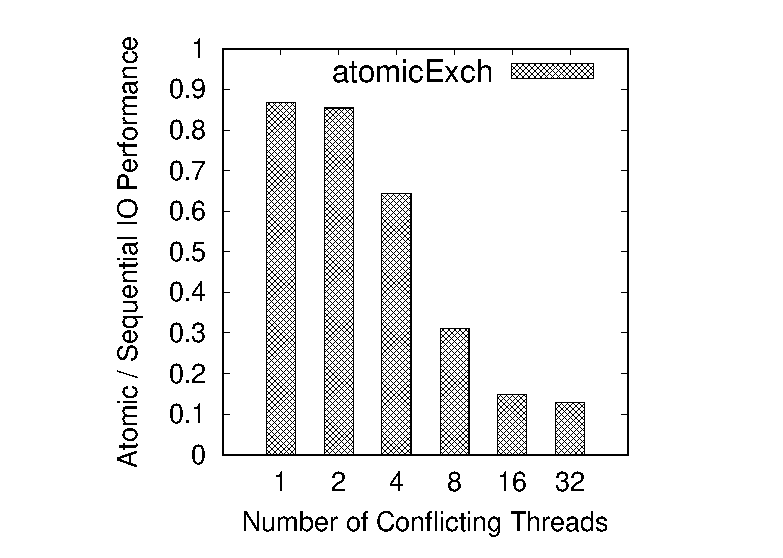
\includegraphics[width=5.3cm]{exp/atomic/atomicExch.eps}
	\end{minipage}
	\caption{The performance of atomic operations for increasing conflicts}
	\label{fig:atomic}
\end{figure}

\vspace{1mm}\noindent\textbf{Find.} It is relative straightforward to parallelize \formal{find} operations as only read access is required. 
Given a batch of size $m$, we launch $w$ warps (meaning we launch $32w$ threads), with each warp being responsible for $\floor{\frac{m}{w}}$ \formal{find} operations. To locate a KV pair, we hash the key to a hash table pair $(h_i,h_j)$ and perform a maximum of two lookups in the corresponding buckets of $h_i$ and $h_j$ respectively. 
%Algorithm~\ref{algo:find} presents the pseudo code for a KV lookup by a warp. 
%First, the bucket of the $i$th hash table is located, i.e., $loc_i$.
%Then, each thread in the warp (a thread lane $l$) simultaneously searches the key and the ballot function return the lane for which the key is found.




\vspace{1mm}\noindent\textbf{Insert.} Contention occurs when multiple \formal{insert} operations target at the same bucket. 
There are two contrasting objectives for resolving contention. On one hand, we want to utilize a warp-centric approach to access a bucket.
On the other hand, when updating a bucket, a warp requires a mutex to avoid corruption, and on GPUs locking is expensive.  
In the literature, it is a common practice to use atomic operations for implementing a mutex under a warp-centric approach \cite{zhang2015mega}. 
We can still invoke a warp to insert a KV pair; however, the warp must acquire a lock before updating the corresponding bucket. 
The warp will keep trying to acquire the lock before successfully obtain control. 
There are two drawbacks to this direct warp-centric approach. 
First, the conflicting warps spin while locking, thus wasting computing resources.
Second, although atomic operations are natively supported by recent GPU architectures, 
they become costly when the number of atomic operations issued at the same location increases. 
In Figure~\ref{fig:atomic}, we show the profiling statistics for two atomic operations that are often used to lock and unlock a mutex: atomicCAS and atomicExch, respectively. 
We compare the throughputs of the atomic operations against an equivalent amount of sequential device memory IOs (coalesced) and present the trend for varying the number of conflicting atomic operations. It is apparent that the atomic performance seriously degrades when a larger number of conflicts occur. 
Thus, it will be expensive for the direct warp-centric approach in contention critical cases. 
Suppose that one wants to track the number of retweets posted to active Twitter accounts in the current month by storing the Twitter ID and the obtained retweet counts as KV pairs. In this scenario, certain Twitter celebrities could receive thousands of retweets in a very short period. 
This causes the same Twitter ID to get updated frequently, thus a large number of conflicts would happen. 




To alleviate the cost of spinning, we devise a voter coordination scheme. 
We assign an \formal{insert} to a thread rather than directly assigning the operation to a warp. Before submitting a locking request and updating the corresponding bucket, the thread will participate in a vote among threads within the same warp. 
The winning thread $l$ becomes the leader of the warp and takes control. Subsequently, the warp inspects the bucket and inserts the KV pair in $l$ if there are spaces left once $l$ has successfully obtained the lock.
If $l$ fails to get the lock, the warp votes for another leader to avoid locking on the same bucket.
Compared with locking in atomic operations, the cost of warp voting is almost negligible as it is heavily optimized in GPU architecture.  


\begin{algorithm}[t]
	\begin{algorithmic}[1]
		\State $active \gets 1$	\label{algo:insert:active:start}
		\While{true}
		\State $l' \gets ballot(active == 1)$ \label{algo:insert:vote:start}
		\If{$l'$ is invalid}
		\State break \label{algo:insert:active:end}
		\EndIf
		\State $[(k',v'),i'] \gets broadcast(l')$ \label{algo:insert:lock:start}
		\State $loc = h^{i'}(k')$
		\If{$l' == l$}
		\State $success \gets lock(loc)$ \label{algo:insert:lock:end}
		\EndIf
		\If{$broadcast(success,l') ==$ failure}
		\State continue					\label{algo:insert:vote:end}
		\EndIf
		\State $l^* \gets ballot(loc[l].key == k' || loc[l].key ==\emptyset)$ \label{algo:insert:write:start}
		\If{$l^*$ is valid and $l' == l$}
		\State $loc[l^*].(key,val) \gets (k',v')$
		\State $unlock(loc)$
		\State $active \gets 0$;
		\State continue			\label{algo:insert:write:end}
		\EndIf
		\State $l^* \gets ballot(loc[l].key \neq \emptyset)$
		\If{$l^*$ is valid and $l' == l$}
		\State $swap(loc[l^*].(key,val),(k',v'))$
		\State $unlock(loc)$ \label{algo:insert:loop:end}
		\EndIf
		\EndWhile
	\end{algorithmic}
	\caption{\textbf{Insert}(lane $l$, warp $wid$)}\label{algo:insert}
\end{algorithm}

Parallel insertions with the voter coordination scheme is presented in Algorithm~\ref{algo:insert}.
The pseudocode in Algorithm~\ref{algo:insert} demonstrates how a thread (with lane $l$) from warp $wid$ inserts a KV pair. 
\revise{The warp first conducts a vote among active threads using the ballot function and the process terminates if all threads finish their tasks} (lines~\ref{algo:insert:active:start}-\ref{algo:insert:active:end}).  
This achieves better resource utilization as no thread will be idle when another thread in the same warp is active.  
The leader $l'$ then broadcasts its KV pair $(k',v')$ and the hash table $h_{i'}$ to the warp and attempts to lock the inserting bucket (lines~\ref{algo:insert:lock:start}-\ref{algo:insert:lock:end}). 
\revise{The ballot and broadcast functions are implemented using the CUDA warp-level primitives $\_\_ballot$ and $\_\_shfl$~\footnote{https://devblogs.nvidia.com/using-cuda-warp-level-primitives/}.}
The broadcast function ensures that all threads in the warp receive the locking result, and if $l'$ fails to obtain a lock, the warp revotes.
Otherwise, the warp follows $l'$ and proceeds to update the bucket for $(k',v')$ with a warp-centric approach like \formal{find}.
Once a thread finds $k'$ or an empty space in the bucket, $l'$ adds or updates it with $(k',v')$ (lines~\ref{algo:insert:write:start}-\ref{algo:insert:write:end}).
If no empty slot is found, $l'$ swaps $(k',v')$ with another KV pair $(k^*,v^*)$ in the bucket and inserts the evicted KV pair to hash table $j$ in the next round. 
The warp finishes the process when all KV pairs have been inserted.
%In summary, each iteration of the loop presented in Algorithm~\ref{algo:insert} issues $1$ atomic operation and at most $1$ device memory read/write (lines~\ref{algo:insert:vote:start}-\ref{algo:insert:loop:end}).  

\vspace{1mm}
\revise{
\noindent\textbf{Implementation Details.} We use atomicCAS and atomicExch functions to lock and unlock buckets, respectively.
The function $atomicCAS(address,compare,val)$ reads the value $old$ located at the address $address$ in global or shared memory and computes $old == compare \;?\; val : old$, and stores the result back to memory at the same address. The function returns the value $old$. The function $atomicExch(address,val)$ reads the value $old$ located at the address $address$ in the global or shared memory and stores $val$ back to memory at the same address. 
To implement the lock, we initialize a lock variable known as $lock$ for each bucket with a value of $0$. 
We lock the bucket using the function $atomicCAS(\&lock,0,1)$, which is successful if the function returns $0$.
Similarly, we unlock the bucket using the function $atomicExch(\&lock,0)$. 
}

%Note that we have yet covered how to choose the hash table index $i$ for each insertion (Algorithm~\ref{algo:insert}). Additional number of conflicts would happen if all threads attempting to insert to the same table. For the flow of presentation, we leave the discussion to Section~\ref{sec:dyn} since choosing the hash table is more coherent to the load balancing problem for resizing hash tables. 
%Moreover, a careful reader would find that the insertion process could lead to multiple appearances of the same key in different hash tables. To fill this gap, one can attach a timestamp to the insertion batch.
%Hence, the \formal{find} operation is required to scan all $d$ buckets of the same key and extracts the one with the latest timestamp.




The following example demonstrates the parallel insertion process.
\begin{example}
	In Figure~\ref{fig:voter}, we visualize a scenario for three threads: $l_x$, $l_y$, $l_z$ from warp $a$ and warp $b$, which insert KV pairs $(k_1,v_1)$, $(k_{33},v_{33})$, and $(k_{65},v_{65})$ independently. 
	Suppose that $l_y$ and $l_z$ become the leaders of warp $a$ and $b$, respectively. Both threads will compete for bucket $y$ and $l_z$ wins the battle. 
	$l_z$ then leads warp $b$ to inspect the bucket and evict KV pair $(k_{64},v_{64})$ by replacing it with $(k_{65},v_{65})$. 
	In the meantime, $l_y$ does not lock bucket $y$ and the new leader $l_x$ is voted in warp $a$. 
	Thread $l_x$ locks bucket $x$ and inserts KV pair $(k_1,v_1)$ in place. Subsequently, $l_y$ may regain the control of warp $a$ and update $k_{33}$ with $(k_{33},v_{33})$ at bucket $y$. In parallel, $l_z$ locks bucket $z$ and inserts the evicted KV $(k_{64},v_{64})$ into the empty space. 
\end{example}

\vspace{1mm}\noindent\textbf{Delete.} 
In contrast with \formal{insert}, the \formal{delete} operation does not require locking with a warp-centric approach. 
As with \formal{find}, we assign a warp to process a key $k$ on deletion. The warp iterates through the buckets of all $d$ hash tables that could possibly contain $k$. Each thread lane in the warp is responsible for inspecting one position in a bucket independently, and erasing the key only if $k$ is found, thus causing no conflict.

%\begin{algorithm}[t]
%	\begin{algorithmic}[1]
%		\For{$i=1,\ldots,d$}
%			\State $loc \gets h^i(k)$
%			\State $found \gets (loc[l].key == k)$
%			\If{$found$}
%				\State $loc[l].key \gets \emptyset$
%			\EndIf
%		\EndFor
%	\end{algorithmic}
%	\caption{\textbf{Delete}(lane $l$, warp $wid$, key $k$)}\label{algo:delete}
%\end{algorithm}


\begin{figure}[t]
	\centering
	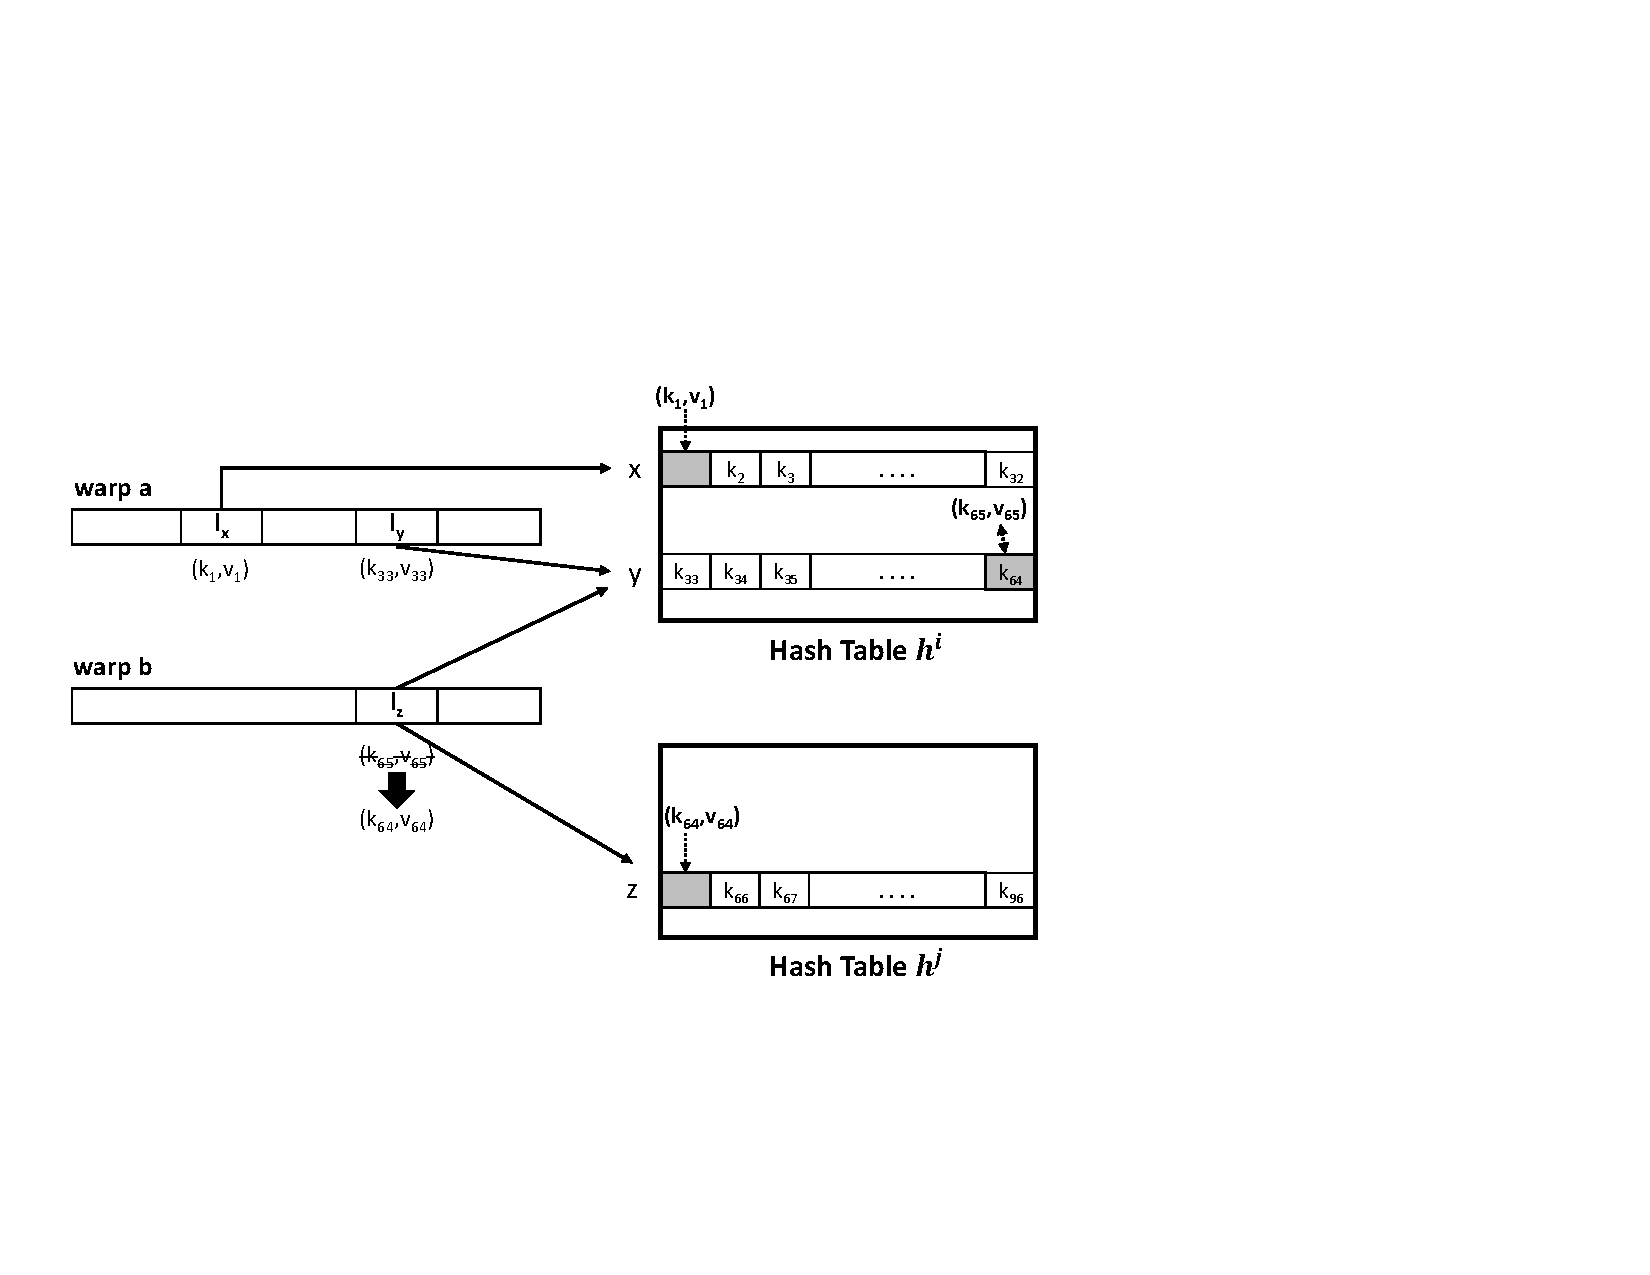
\includegraphics[width=0.48\textwidth]{fig/Voter.pdf}
	\vspace{-1em}
	\caption{Example for parallel insertions}
	\label{fig:voter}
\end{figure}
\vspace{1mm}\noindent\textbf{Complexity.}
Because \formal{find}, \formal{insert} and \formal{delete} operations are independently executed by threads, 
the analysis of a single thread's complexity is the same as in the sequential version of cuckoo hashing \cite{pagh2004cuckoo}: $O(1)$ worst case complexity for \formal{find} and \formal{delete}, $O(1)$ expected time for \formal{insert} for the case of two hash tables. 
It has been pointed out that analyzing the theoretical upper bound complexity of insertion in $d \geq 3$ hash tables is difficult \cite{alcantara2009real}.  
Nevertheless, empirical results have shown that increasing the number of tables leads to better insertion performance. Please refer to the experimental results presented in Section~\ref{sec:exp}.
%Thus, we assume the complexity for inserting to $d$ hash tables is the same as that of $2$ has tables, as long as $d$ keeps constant.  

We then analyze the number of possible thread conflicts. Assuming we launch $m$ threads in parallel, each thread is assigned to a unique key, and the total number of unique buckets is $H=\sum_{i=1}^d|h^i|$. For \formal{find} and \formal{delete}, there is no conflict at all. 
For \formal{insert}, computing the expected number of conflicting buckets resembles the \emph{balls and bins} problem \cite{raab1998balls}, which is $O(\binom{m}{2}/H)$. 
Given that GPUs have many threads, there could be a significant amount of conflicts. Thus, we propose the voter coordination scheme to reduce the cost of spinning in locks. 
%Note that the analysis is done for the cases where the key to update is unique. More conflicts could occur in reality when the same key is updated in parallel. 